\begin{GreyBox}
    \vskip-1cm
    \begin{block}{\GHead{Results}} 
        
        \begin{center}
            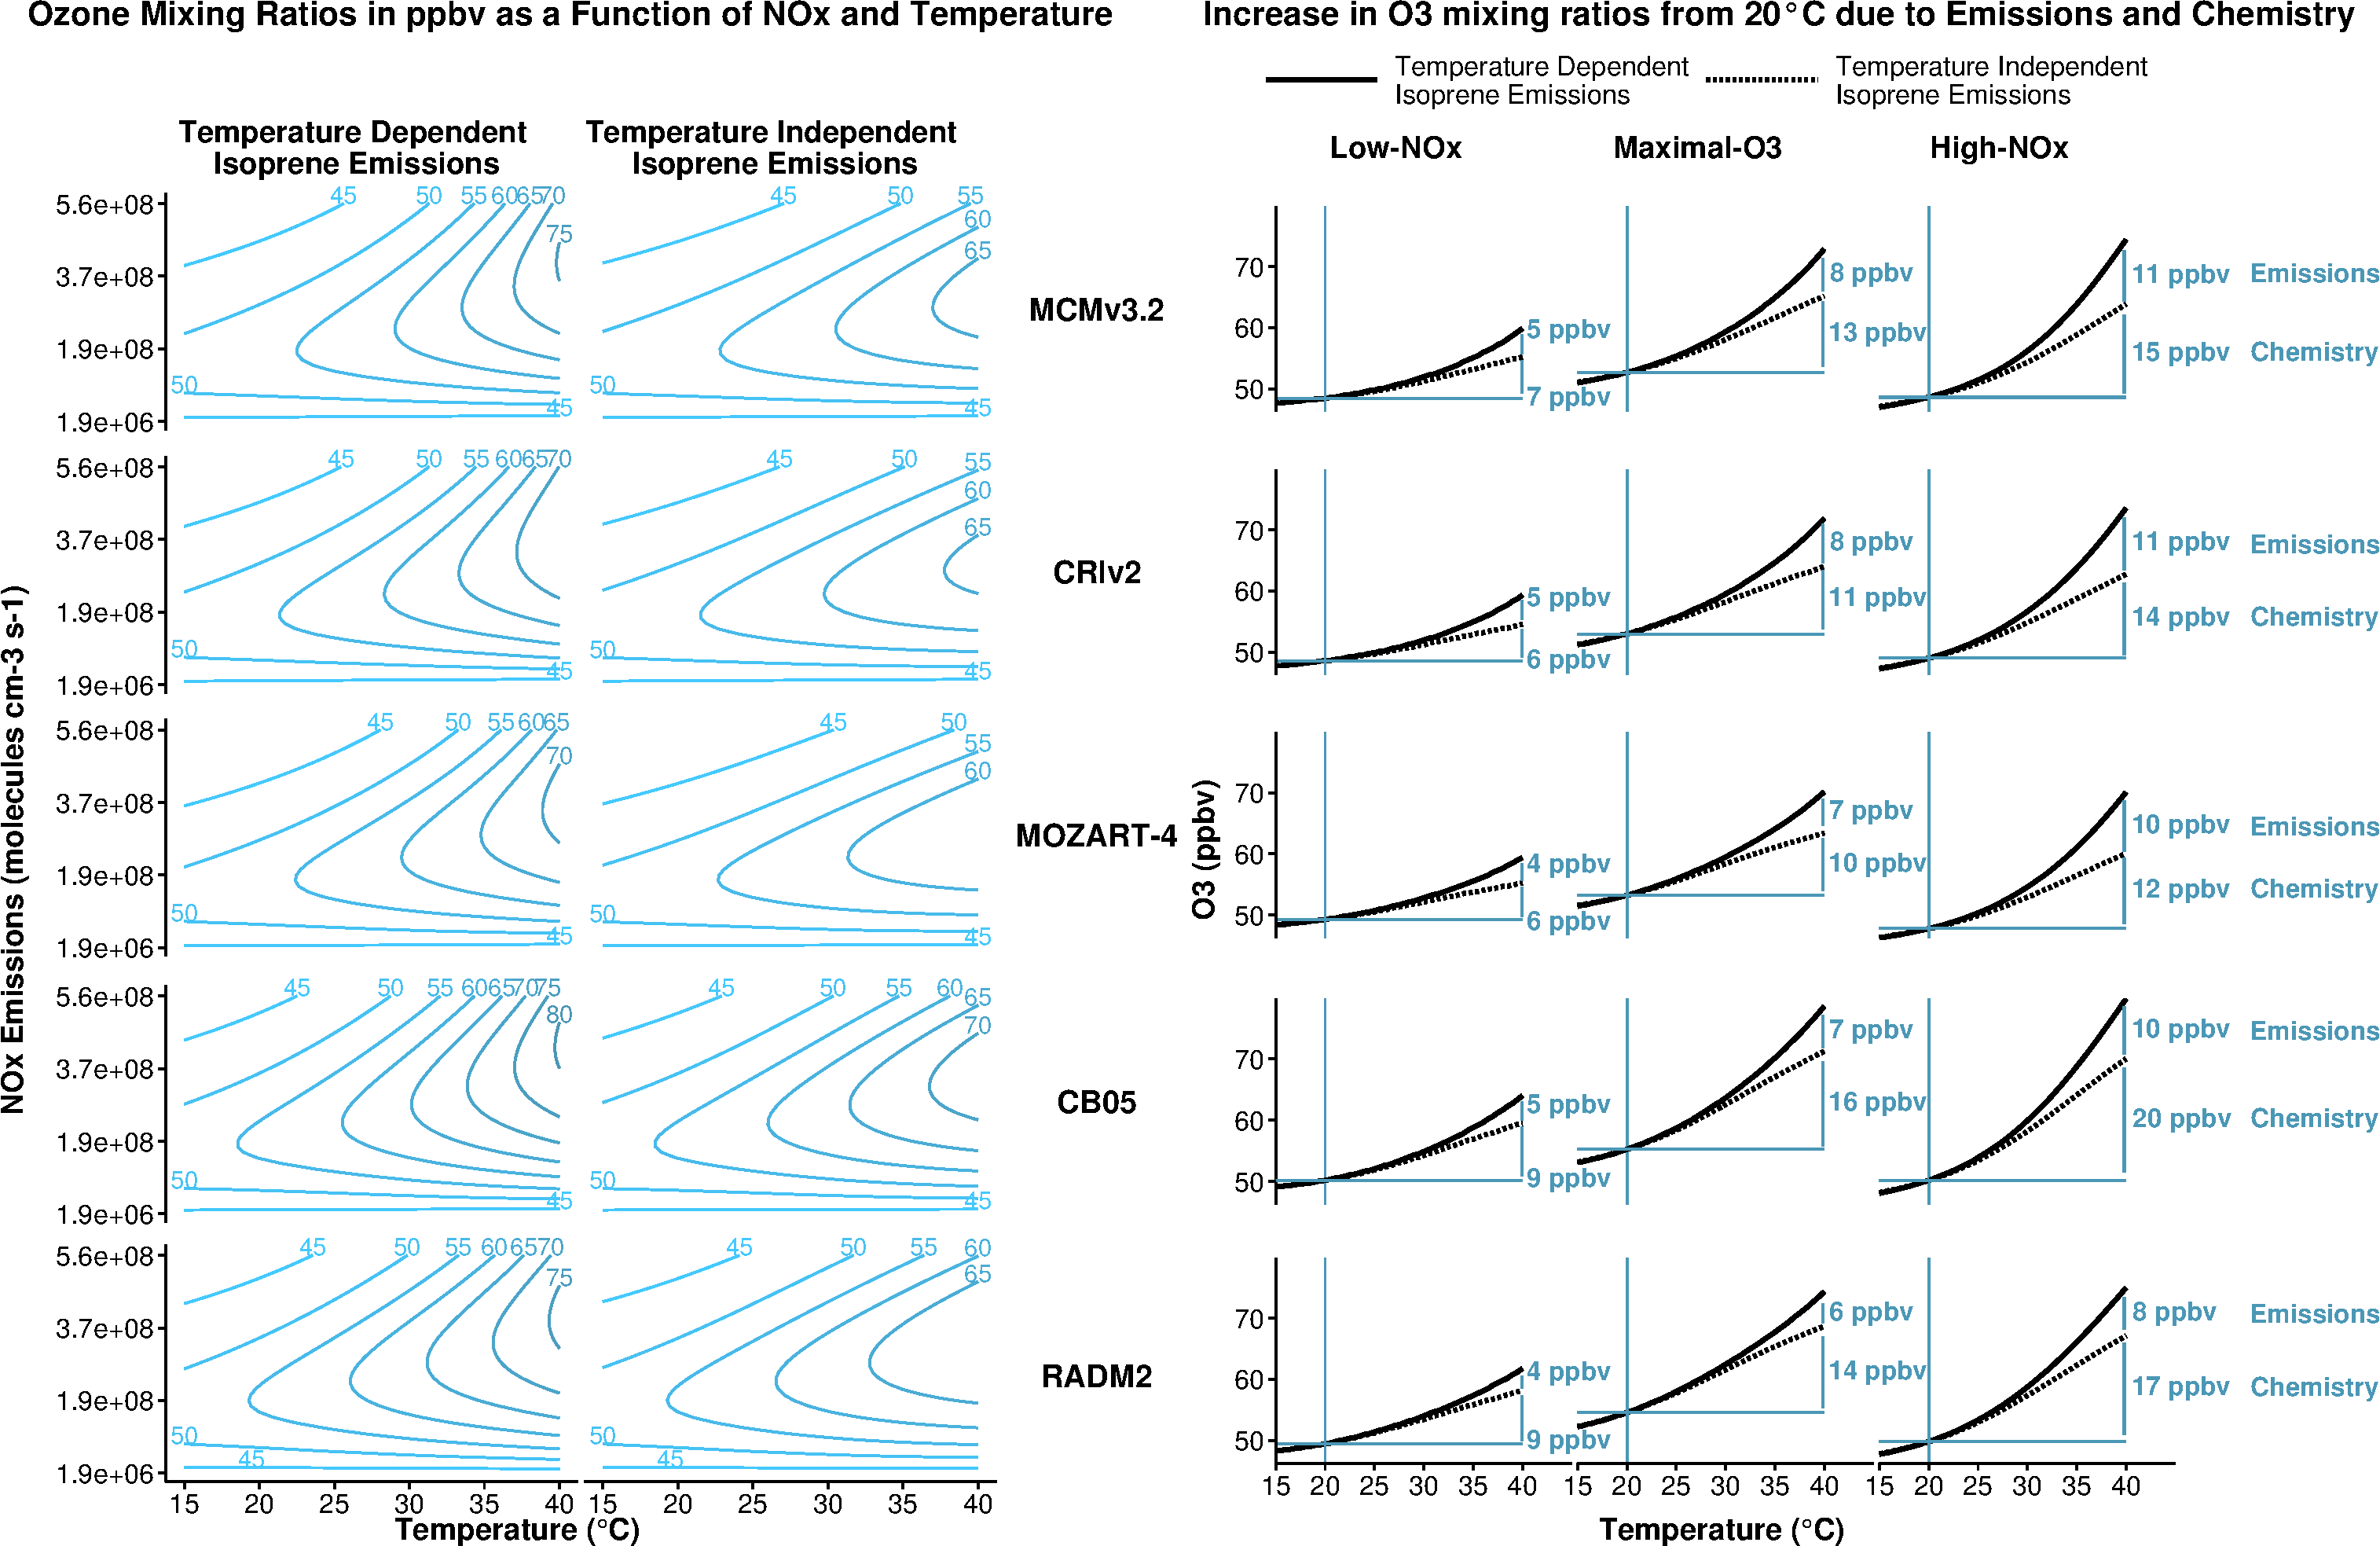
\includegraphics[width=\textwidth]{Plotting/results}
        \end{center}
        \begin{columns}[c]
            \column{0.45\textwidth}
                %\includegraphics[width=\textwidth]{img/O3_comparison}
                %\vskip3cm
                \begin{WhiteBox}
                    \begin{itemize} \vspace{3mm}
                        \item Non-linear relationship of ozone mixing ratios with \ce{NO_x} and temperature, reproduced by all chemical mechanisms. \vspace{9mm}
                        \item Higher ozone produced using RADM2 and CB05 compared to detailed chemistry of MCMv3.2. \vspace{9mm}
                        \item Increased ozone when including temperature dependent source of isoprene, especially at high-\ce{NO_x}. \vspace{9mm}
                        \item Lower \ce{NO_x} levels have lowest ozone mixing ratios with both temperature dependent and independent source of isoprene. \vspace{9mm}
                    \end{itemize}
                \end{WhiteBox}
            \column{0.45\textwidth}
                %\includegraphics[width=\textwidth]{img/Ox_budgets_Contributions}
                %\vskip3cm
                \begin{WhiteBox} \vspace{3mm}
                    \begin{itemize}
                        %\item Assigned the ozone produced to three \ce{NO_x}-regimes based on \ce{H2O2}/\ce{HNO3}. \vspace{9mm}
                        %\item The contributions of the reactions of peroxy radicals with NO to \ce{O_x} (= \ce{O3 + NO2}) production budgets are determined for each \ce{NO_x}-condition.\vspace{9mm}
                        \item Contributions of methyl peroxy (\ce{CH3O2}) and acyl peroxy (\ce{CH3CO3}) to \ce{O_x} budget increases with temperature.\vspace{9mm}
                        \item \ce{CH3CO3} is a precursor of \ce{CH3O2} which in turn is a precursor of \ce{HO2}. Thus increased source of a precursor of \ce{CH3CO3} - acetaldehyde - leads to higher ozone production.\vspace{9mm}
                        \item Acetaldehyde is an important carbonyl product, especially during isoprene degradation, and in CB05 and RADM2 it as a much higher yield, due to a lack of representation or underestimation of the ketone yield from VOC oxidation.\vspace{9mm}
                    \end{itemize}
                \end{WhiteBox}
        \end{columns}
    \end{block}
\end{GreyBox}
